\documentclass{article}

\makeatletter
\renewcommand{\fnum@figure}{Εικόνα \thefigure}
\makeatother

\usepackage[greek, english]{babel}
\usepackage{alphabeta}
\usepackage{atbegshi, picture}

% Set page size and margins
% Replace `letterpaper' with`a4paper' for UK/EU standard size
\usepackage[letterpaper,top=2cm,bottom=2cm,left=3cm,right=3cm,marginparwidth=1.75cm]{geometry}

% Useful packages
\usepackage{amsmath}
\usepackage{graphicx}
\usepackage[colorlinks=true, allcolors=blue]{hyperref}
\usepackage[utf8]{inputenc}
\usepackage{indentfirst}

\newcommand\T{\rule{0pt}{2.6ex}}       % Top strut
\newcommand\B{\rule[-1.2ex]{0pt}{0pt}} 


\addto\captionsenglish{
  \renewcommand{\contentsname}
    {Περιεχόμενα}
}

% \title{Feasibility Study}
% \date{}

\begin{document}
% \maketitle

\begin{titlepage}
   \begin{center}
       \vspace*{1cm}

       \textbf{\huge Use Cases}

       \vspace{0.5cm}
        Τεχνολογία Λογισμικού
            
       \vspace{1cm}

       \textbf{Αγγελική Κούρου\\Κατερίνα Μητροπούλου}
       
       \begin{figure}[!htb]
        \centering
        
\includegraphics[width=0.5\textwidth]{logo.png}
        \end{figure}
        
        \vspace{0.5cm}
        
        \begin{figure}[!htb]
        \centering
        \includegraphics[width=0.5\textwidth]{UoP.jpg}
        \end{figure}


       \vfill
            
       Τεχνικό Κείμενο για την Τεχνολογία Λογισμικού\\
            
       \vspace{0.5cm}
            
       CEID, ECE\\
       University of Patras\\
            
   \end{center}
\end{titlepage}



\noindent Η ομάδα μας

\begin{enumerate}
  \item Βεργίνης Δημήτριος, ΑΜ: 1066634 , ECE
  \item Βλαχογιάννης Δημήτριος, ΑΜ: 1067371, CEID
  \item Κούρου Αγγελική, ΑΜ: 1067499 , CEID
  \item Μητροπούλου Αικατερίνα - Quality Manager, ΑΜ: 1067409, CEID
  \item Στεφανίδης Μάριος - Project Manager, ΑΜ:1067458, CEID
\end{enumerate}

{
  \hypersetup{linkcolor=black}
  \tableofcontents
}

\newpage

\section{Εισαγωγή}

Τα Use Cases αποτελούν ένα σύνολο δραστηριοτήτων ή βημάτων που λαμβάνουν χώρα κατά την πλοήγηση ενός χρήστη (ή ρόλου, γνωστού στην UML ως ηθοποιού) σε ένα σύστημα, για να επιτευχθεί ένας στόχος. Ο ηθοποιός μπορεί να είναι άνθρωπος ή κάποιο άλλο εξωτερικό σύστημα. 
Για την ανάπτυξη ενός use case χρησιμοποιούνται τα διαγράμματα περιπτώσεων χρήσης, καθώς και λεκτική περιγραφή των περιπτώσεων αυτών.

\section{Διάγραμμα Περιπτώσεων Χρήσης}

Παρακάτω παρουσιάζεται το διάγραμμα περιπτώσεων χρήσης. Για την καλύτερη κατανόηση του διαγράμματος σημειώνεται ότι:

\begin{enumerate}
  \item Τα σκίτσα με τους ανθρώπους αντιστοιχούν στους ηθοποιούς του εκάστοτε use case, δηλαδή τους εμπλεκόμενους
  \item Οι μπλε ελλείψεις αντιστοιχούν στα use cases
  \item Οι μαύρες γραμμές απεικονίζουν άμεση συσχέτιση μεταξύ ενός ηθοποιού και μίας περίπτωσης χρήσης
  \item Οι μπλε διακεκομμένες γραμμές (το μπλε επιλέχθηκε για ευαναγνωσία) απεικονίζουν τη σχέση εξάρτησης μεταξύ δύο περιπτώσεων χρήσης, δηλαδή το use case στο οποίο δείχνει το βέλος δεν μπορεί να υπάρξει αν δεν έχει προηγηθεί το use case από το οποίο ξεκινάει το βέλος  
\end{enumerate}


\underline{Σημείωση}: Στο παρακάτω διάγραμμα, ενώ το use case που αφορά στην διαδικασία log in, είναι προαπαιτούμενο για την ύπαρξη όλων των υπολοίπων, δεν παριστάνονται οι συγκεκριμένες συσχετίσεις εξάρτησης για την καλύτερη παρουσασίαση και ευαναγνωσία του διαγράμματος.

\newpage

\begin{figure}[!htb]
        \centering
        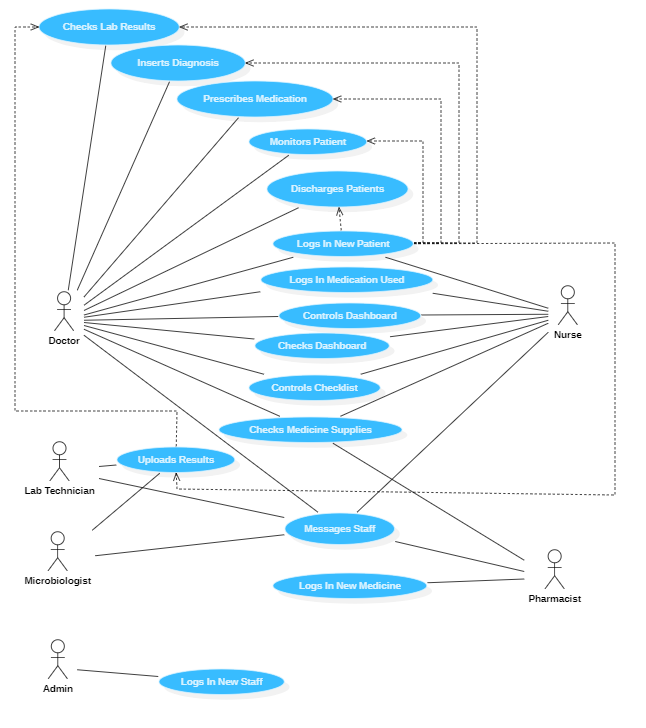
\includegraphics[width=1.0\textwidth]{UML.png}
        \caption{\label{fig: UML} Use Case Diagram}
\end{figure}
        
\vspace{0.5cm}

Για τις παρακάτω περιπτώσεις χρήσης δεν αναγράφονται στους πίνακες τα παρακάτω ως \par προαπαιτούμενα χάριν συντομίας:

\begin{enumerate}
    \item  Ο χρήστης να έχει καταχωρηθεί στο σύστημα
    \item Ο χρήστης να έχει συνδεθεί στο \textbf{Medic World}
\end{enumerate}


\section{Use Case 1: Διάγνωση Ασθενούς}

Παρακάτω θα αναλυθεί το σενάριο χρήσης του \textbf{Medic World}, στο οποίο ένας γιατρός καταχωρεί την διάγνωση στην καρτέλα ενός ασθενούς.

\subsection{Περιγραφή}

\begin{center}
     \begin{tabular}{|l|l|}
     \hline
      \textbf{Περίπτωση Χρήσης 1} & Ο γιατρός εισάγει τη διάγνωση ενός ασθενούς \T\B \\ 
      \hline
      \textbf{Ηθοποιός} & Γιατρός \T\B \\
      \hline
      \textbf{Σενάριο Περίπτωσης Χρήσης} & Ένας από τους ασθενείς χρείαζεται διάγνωση, οπότε \T\\& ο γιατρός εισέρχεται στην καρτέλα του, μελετάει τα\\& αποτελέσματα των εξετάσεών και συμπτώματα του και \\& καταλήγει σε διάγνωση \B \\
      \hline
      \textbf{Αφορμή} & Ασθενής χρειάζεται διάγνωση \T\B \\
      \hline
      \textbf{Προαπαιτούμενο 1} & Να έχει καταχωρηθεί ο ασθενής στο σύστημα \T\B \\
      \hline
      \textbf{Προαπαιτούμενο 2} & Να είναι έτοιμα τα αποτελέσματα των εργαστηριακών εξετάσεων \T\B \\
      \hline
     \end{tabular}
 \end{center}
 
 \subsection{Αναλυτικό Σενάριο Χρήσης}
 
 \begin{center}
     \begin{tabular}{|l|l|}
     \hline
      \textbf{Περιγραφή} & Αυτό το σενάριο περιγράφει μια κατάσταση όπου χρειάζεται \T \\& η πλοήγηση σε τέσσερις καρτέλες, οι οποίες τελικά\\& οδηγούν στην επίτευξη του στόχου. \B \\ 
      \hline
      \textbf{Βήμα 1} & Ο γιατρός από το κεντρικό μενού επιλέγει το εικονίδιο \T \\& "Patients" και το σύστημα τον κατευθύνει στην λίστα των ασθενών \B \\
      \hline
      \textbf{Βήμα 2} & Πλοηγείται στην καρτέλα και επιλέγοντας το όνομα του ασθενούς \T \\& κατευθύνεται στο προφίλ του  \B \\
      \hline
      \textbf{Βήμα 3} & Ανανεώνονται και εμφανίζονται οι τρέχουσες ζωτικές ενδείξεις του ασθενούς \T\B \\
      \hline
      \textbf{Βήμα 4} & Επιλέγοντας την ένδειξη "Patient's Profile" κατευθύνεται στο \T\\& ιστορικό του ασθενούς, το οποίο και μελετάει \B \\
      \hline
      \textbf{Βήμα 5} & Επιλέγοντας την ένδειξη "Lab Results" κατευθύνεται \T \\& στα αποτελέσματα εξετάσεων του ασθενούς \B \\
      \hline
      \textbf{Βήμα 6} & Επιλέγει τις εικόνες των εξετάσεων, για να τις μελετήσει \T\B \\
      \hline
      \textbf{Βήμα 7} & Επιλέγοντας την ένδειξη "Diagnosis" εμφανίζεται αναδυόμενο \T \\& παράθυρο με πιθανές ασθένειες \B \\
      \hline
      \textbf{Βήμα 8} & Μελετά την λίστα και επιλέγει την αντίστοιχη ασθένεια\T\B \\
      \hline      
      \textbf{Βήμα 9} & Κατευθύνεται στο παράθυρο ολοκλήρωσης της διάγνωσης \T\B \\
      \hline
      \textbf{Βήμα 10} & Εφαρμόζει τις κατάλληλες τροποποιήσεις \T\B \\
      \hline
      \textbf{Βήμα 11} & Πατάει το κουμπί επιβεβαίωσης \T\B \\
      \hline
      \textbf{Βήμα 12} & Εμφανίζεται αναδυόμενο παράθυρο με την ένδειξη "Sucessful" \T\B \\
      \hline    
      \textbf{Βήμα 13} & Επιλέγει το κουμπί "ΟΚ"\T\B \\ 
      \hline
      \textbf{Βήμα 14} & Ενημερώνεται το σύστημα και το προφίλ του ασθενούς \T\B \\
      \hline
     \end{tabular}
 \end{center}
 
 \vspace{0.1cm}
 
 \textbf{\underline{Εναλλακτική Ροή}:} \vspace{0.005cm} \\
\par \textbf{Βήμα 8.1:} Δεν τον ικανοποιεί η λίστα των πιθανών ασθενειών, επομένως \parεπιλέγει την έξοδο από το παράθυρο.\\
\par \textbf{Βήμα 9.1:} Κατευθύνεται στο παράθυρο ολοκλήρωσης της διάγνωσης.\\
\par \textbf{Βήμα 10.1:} Εισάγει τη διάγνωση του. \\

 
 \section{Use Case 2: Απασχόληση Χειρουργείου}
 
 Παρακάτω θα αναλυθεί το σενάριο χρήσης του \textbf{Medic World}, στο οποίο ένας χρήστης επιθυμεί να δηλώσει στο σύστημα τη χρήση ενός χειρουργείου.

\subsection{Περιγραφή}

\begin{center}
     \begin{tabular}{|l|l|}
     \hline
      \textbf{Περίπτωση Χρήσης 2} & Ο χρήστης δηλώνει την απασχόληση χειρουργείου \T\B \\ 
      \hline
      \textbf{Ηθοποιός} & Γιατρός \T\B \\
      \hline
      \textbf{Σενάριο Περίπτωσης Χρήσης} & Ένας γιατρός πρόκειται να εισάγει έναν ασθενή \T \\& σε κάποιο χειρουργείο και χρειάζεται να καταχωρηθεί\\& στην καρτέλα των χειρουργείων ότι το συγκεκριμένο\\& δωμάτιο δε θα είναι διαθέσιμο για κάποιο χρονικό διάστημα \B \\
      \hline
      \textbf{Ηθοποιοί} & Γιατρός, Νοσηλευτής \T\B \\
      \hline
      \textbf{Αφορμή} & Ασθενής χρειάζεται χειρουργείο \T\B \\
      \hline
      \textbf{Προαπαιτούμενο 1} & Να έχει καταχωρηθεί ο ασθενής στο σύστημα \T\B \\
      \hline
      \textbf{Πρoαπαιτούμενο 2} & Να έχει πραγματοποιηθεί διάγνωση του ασθενούς \T\B \\
      \hline
      \textbf{Προαπαιτούμενο 3} & Η διάγνωση να απαιτεί την εισαγωγή σε χειρουργείο \T\B \\
      \hline
     \end{tabular}
 \end{center}
 
 \subsection{Αναλυτικό Σενάριο Χρήσης}
 
 \begin{center}
     \begin{tabular}{|l|l|}
     \hline
      \textbf{Περιγραφή} & Αυτό το σενάριο περιγράφει μια κατάσταση όπου χρείαζεται \T \\& η πλοήγηση σε τρεις καρτέλες, οι οποίες οδηγούν στην \\& επίτευξη του στόχου. \B \\ 
      \hline
      \textbf{Βήμα 1} & Ο χρήστης από το κεντρικό μενού επιλέγει το εικονίδιο  ”Checklist" \T \\& και το σύστημα τον κατευθύνει στην αντίστοιχη οθόνη \B \\
      \hline
      \textbf{Βήμα 2} & Ο χρήστης επιλέγει από το μενού του Checklist \T  τα "Operating Rooms" \T \\& και οδηγείται σε οθόνη που εμφανίζονται όλα τα χειρουργεία διαθέσιμα\\& και μη, με τις αντίστοιχες ενδείξεις \B \\
      \hline
      \textbf{Βήμα 3} & Ο χρήστης ελέγχει την διαθεσιμότητα των χειρουργείων και επιλέγει ένα από τα διαθέσιμα \T\B \\
      \hline
      \textbf{Βήμα 4} & Ο χρήστης οδηγείται σε μία φόρμα συμπλήρωσης στοιχείων \T\B \\
      \hline
      \textbf{Βήμα 5} & Πληκτρολογώντας το όνομα του γιατρού στον χρήστη εμφανίζονται προτάσεις \T \\& από χειρούργους γιατρούς ήδη καταγεγραμμένους στο σύστημα \B \\
      \hline
      \textbf{Βήμα 6} & Πληκτρολογώντας το όνομα του ασθενούς στον χρήστη εμφανίζονται προτάσεις \T \\& από ασθενείς ήδη καταχωρημένους στο σύστημα \B \\
      \hline      
      \textbf{Βήμα 7} & Ο χρήστης πληκτρολογεί την εγχείρηση που πρόκειται να πραγματοποιηθεί \T\B \\   
      \hline
      \textbf{Βήμα 8} & Ο χρήστης μέσω του πλήκτρου "Done" επιλέγει την \T \\& ολοκλήρωση της διαδικασίας \B \\
      \hline
      \textbf{Βήμα 9} & Εμφανίζεται αναδυόμενο παράθυρο με την ένδειξη "Successful" \T\B \\
      \hline
      \textbf{Βήμα 10} & Ενημερώνεται το σύστημα και στην καρτέλα διαθεσιμότητας των χειρουργείων \T \\& εμφανίζεται πλέον ως μη διαθέσιμο το χειρουργείο που επέλεξε νωρίτερα ο χρήστης \B \\
      \hline
     \end{tabular}
 \end{center}
 
\newpage
 
\textbf{\underline{Εναλλακτική Ροή 1}:} \vspace{0.005cm} \\
\par \textbf{Βήμα 7.1:} O ασθενής δεν είναι καταγεγραμμένος στο σύστημα (παραδείγματος χάριν λόγω επείγοντως \par περιστατικού), επομένως καταχωρείται η επιλογή "not registered".

\vspace{0.3cm}

\textbf{\underline{Εναλλακτική Ροή 2}:} \vspace{0.005cm} \\
\par \textbf{Βήμα 8.2:} Πληκτρολογεί λανθασμένα την εγχείρηση και το σύστημα του εμφανίζει πιθανές διορθώσεις, \par από τις οποίες μπορεί να επιλέξει κάποια, αν το επιθυμεί. 

\section{Use Case 3: Καταχώρηση Νέου Φαρμάκου }
 
 Παρακάτω θα αναλυθεί το σενάριο χρήσης του \textbf{Medic World} κατά το οποίο ένας φαρμακοποιός επιθυμεί να εισάγει στο σύστημα ένα νέο φάρμακο.
 
\subsection{Περιγραφή}

\begin{center}
     \begin{tabular}{|l|l|}
     \hline
      \textbf{Περίπτωση Χρήσης 3} & Ο χρήστης εισάγει νέο φάρμακο στην καρτέλα προμηθειών \T\B \\ 
      \hline
      \textbf{Ηθοποιός} & Φαρμακοποιός \T\B \\
      \hline
      \textbf{Σενάριο Περίπτωσης Χρήσης} & Έχει γίνει από το νοσοκομείο αγορά ενός νέου φαρμάκου \T \\& και ο φαρμακοποιός καλείται να το καταχωρήσει \\& στην καρτέλα προμηθειών \B \\
      \hline
      \textbf{Αφορμή} & Η αγορά νέου φαρμάκου \T\B \\
      \hline
      \textbf{Προαπαιτούμενο 1} &  Να μην υπάρχει ήδη το φάρμακο στην καρτέλα προμηθειών \T\B \\
      \hline
     \end{tabular}
 \end{center}
 
 \subsection{Αναλυτικό Σενάριο Χρήσης}
 
 \begin{center}
     \begin{tabular}{|l|l|}
     \hline
      \textbf{Περιγραφή} & Αυτό το σενάριο περιγράφει μια κατάσταση όπου χρειάζεται \T \\& πλοήγηση σε δύο καρτέλες, οι οποίες οδηγούν στην επίτευξη \\& του στόχου \B \\ 
      \hline
      \textbf{Βήμα 1} & Ο φαρμακοποιός από το κεντρικό μενού επιλέγει το εικονίδιο ”Supplies” \T \\& και το σύστημα τον κατευθύνει στην αντίστοιχη οθόνη\\
      \hline
      \textbf{Βήμα 2} & Επιλέγοντας το πλήκτρο "New Medicine" κατευθύνεται στη φόρμα \T \\& συμπλήρωσης του νέου φαρμάκου \B \\
      \hline
      \textbf{Βήμα 3} & Πληκτρολογώντας τη κατηγορία του φαρμάκου στον χρήστη εμφανίζονται προτάσεις \T \\& από τις υπάρχουσες κατηγορίες (λ.χ. αντιβιοτικό), από τις οποίες πρέπει να επιλέξει κάποια \B \\
      \hline
      \textbf{Βήμα 4} & Ο φαρμακοποιός καταχωρεί το όνομα του φαρμάκου \T\B \\
      \hline
      \textbf{Βήμα 5} &  Ο φαρμακοποιός συμπληρώνει τα τεμάχια που προμηθεύτηκαν \T\B \\
      \hline
      \textbf{Βήμα 6} & Ο φαρμακοποιός καταγράφει τα όρια των τιμών που περιγράφουν την πληρότητα του \T \\& φαρμάκου (αν είναι σε αφθονία κ.ο.κ.)\B \\
      \hline
      \textbf{Βήμα 9} & Ο φαρμακοποιός επιλέγει το κουμπί "Done" \T\B \\
      \hline
      \textbf{Βήμα 10} & Εμφανίζεται αναδυόμενο παράθυρο με την ένδειξη "Successful" \T\B \\
      \hline    
      \textbf{Βήμα 11} & Γίνεται καταχώρηση στο σύστημα και στην καρτέλα διαθεσιμότητας φαρμάκων, \T \\& επιλέγοντας την κατηγορία  που αφορά το νεοεισαχθέν φάρμακο, εμφανίζεται πλέον το νέο προϊόν \B \\
      \hline
     \end{tabular}
 \end{center}
 
 \newpage
 
\textbf{\underline{Εναλλακτική Ροή 1}:} \vspace{0.005cm} \\
\par \textbf{Βήμα 3.1:} Η κατηγορία φαρμάκου που πληκτρολόγησε ο χρήστης δεν υπάρχει στο σύστημα, συνεπώς \par αυτομάτως δημιουργείται νέα κατηγορία.

\vspace{0.3cm}
 
 \textbf{\underline{Εναλλακτική Ροή 2}:} \vspace{0.005cm} \\
\par \textbf{Βήμα 4.2:} Το φάρμακο που συμπλήρωσε ο χρήστης είναι ήδη καταχωρημένο, με αποτέλεσμα \par το σύστημα αυτομάτως να κλειδώνει και να μη του επιτρέπει τη συνέχεια της διαδικασίας εώς ότου \par διορθωθεί το όνομα ή "αποχωρήσει" από την καρτέλα.

\section{Use Case 4: Αποστολή Μηνύματος}

Παρακάτω θα αναλυθεί το σενάριο χρήσης του \textbf{Medic World}, στο οποίο χρήστες της εφαρμογής ανταλλάσσουν μηνύματα μεταξύ τους.

\subsection{Περιγραφή}

\begin{center}
     \begin{tabular}{|l|l|}
     \hline
      \textbf{Περίπτωση Χρήσης 4} & Ο χρήστης στέλνει μήνυμα σε κάποιον άλλο χρήστη της εφαμοργής \T\B \\ 
      \hline
      \textbf{Ηθοποιός} & Γιατρός \T\B \\
      \hline
      \textbf{Σενάριο Περίπτωσης Χρήσης} & Έχει εισαχθεί ένας νέος ασθενής στο νοσοκομείο και επιθυμεί να \T \\& μάθει, αν ένας συνάδελφός του έχει ελέγξει τις εξετάσεις \B \\
      \hline
      \textbf{Ηθοποιοί} & Γιατρός, Νοσηλευτής, Μικροβιολόγος, Υπεύθυνοι Εργαστηρίου, \T \\& Φαρμακοποιός, Διαχειριστής Συστήματος \T\B \\
      \hline
      \textbf{Αφορμή} & Έτοιμες εξετάσεις για έλεγχο \T\B \\
      \hline
      \textbf{Προαπαιτούμενο 1} & Να έχει εισαχθεί ο ασθενής στο σύστημα \T\B \\
      \hline
      \textbf{Προαπαιτούμενο 2} & Να έχει γίνει η παραγγελία των εξετάσεων \T\B \\
      \hline
      \textbf{Προαπαιτούμενο 3} & Να έχουν ολοκληρωθεί οι εξετάσεις \T\B \\
      \hline
     \end{tabular}
 \end{center}

\newpage

\subsection{Αναλυτικό Σενάριο Χρήσης}

 \begin{center}
     \begin{tabular}{|l|l|}
     \hline
      \textbf{Περιγραφή} & Αυτό το σενάριο περιγράφει μια κατάσταση όπου χρειάζεται \T \\& πλοήγηση σε τρεις καρτέλες, οι οποίες οδηγούν στην επίτευξη \\& του στόχου \B \\ 
      \hline
      \textbf{Βήμα 1} & Ο χρήστης από το κεντρικό μενού επιλέγει το εικονίδιο ”Messages” \T \\& και το σύστημα τον κατευθύνει στην αντίστοιχη οθόνη \B \\
      \hline
      \textbf{Βήμα 2} & Επιλέγοντας το εικονίδιο που αντιστοιχεί στην λειτουργία "Σύνταξη \T \\& νέου μηνύματος" κατευθύνεται σε καρτέλα, ώστε να αναζητήσει τον \\& χρήστη που επιθυμεί να στείλει μήνυμα \B \\
      \hline
      \textbf{Βήμα 3} & Πληκτρολογώντας το όνομα του χρήστη εμφανίζονται προτάσεις \T \\& από τους καταχωρημένους στο σύστημα χρήστες, για να επιλέξει τον \\& χρήστη που θέλει να αποστείλει μήνυμα \B \\
      \hline
      \textbf{Βήμα 4} & Πληκτρολογεί το κείμενο στο αντίστοιχο πεδίο \T\B \\
      \hline
      \textbf{Βήμα 5} &  Επιλέγει το εικονίδιο που αντιστοιχεί στην  λειτουργία "Αποστολή μηνύματος"\T\B \\
      \hline
      \textbf{Βήμα 6} & Στον χρήστη εμφανίζεται το περίγραμμα ενός κύκλου που περιέχει ένα τικ, δίπλα \T \\& από το μήνυμά του, το οποίο υποδεικνύει πως το μήνυμα έχει σταλεί αλλά δεν έχει παραδοθεί \B \\
      \hline
      \textbf{Βήμα 7} & Η κατάσταση του μηνύματος ενημερώνεται, αφού ο παραλήπτης το διαβάσει \T\B \\
      \hline
     \end{tabular}
 \end{center}
 
\vspace{0.2cm}
 
\textbf{\underline{Εναλλακτική Ροή 1}:} \newline
\par Ο χρήστης που επιθυμεί να συνομιλήσει, βρίσκεται ήδη στο ιστορικό των συζητήσεων του, επομένως: \newline
\par \textbf{Βήμα 2.1:} Περιηγείται στην οθόνη και επιλέγει την συνομιλία τους ή \newline
\par \textbf{Βήμα 2.2:} Πληκτρολογεί το όνομά του στο πεδίο αναζήτησης και κατευθύνεται απευθείας στην \par συνομιλία τους.


\section{Use case 5: Εντοπισμός και Διαχείριση Βλάβης}

Παρακάτω θα αναλυθεί το σενάριο χρήσης του \textbf{Medic World}, στο οποίο ο διαχειριστής του συστήματος θα λαμβάνει ειδοποίηση σχετικά με τη βλάβη μιας συσκευής και θα δρομολογεί την επιδιόρθωσή της.

\subsection{Περιγραφή}

\begin{center}
     \begin{tabular}{|l|l|}
     \hline
      \textbf{Περίπτωση Χρήσης 5} & Προσθήκη δραστηριότητας στο πρόγραμμά έπειτα από ειδοποίηση \T\B \\
      \hline
      \textbf{Ηθοποιός} & Διαχεριστής Συστήματος \T\B \\
      \hline
      \textbf{Σενάριο Περίπτωσης Χρήσης} &  Ο διαχειριστής του συστήματος λαμβάνει ειδοποίηση πως παρουσιάστηκε \T \\& βλάβη σε κάποια συσκευή και δρομοληγεί την επιδιόρθωσή της \B \\
      \hline
      \textbf{Αφορμή} & Παρουσίαση βλάβης σε συσκευή του δικτύου \T\B \\
      \hline
      \textbf{Προαπαιτούμενο 1} & Η συσκευή να είναι συνδεδέμενη στο δίκτυο \T\B \\
      \hline
     \end{tabular}
 \end{center}
 
\subsection{Αναλυτικό Σενάριο Χρήσης}

 \begin{center}
     \begin{tabular}{|l|l|}
     \hline
      \textbf{Περιγραφή} & Αυτό το σενάριο περιγράφει μια κατάσταση όπου χρειάζεται \T \\& πλοήγηση σε μία καρτέλα, οι οποίες οδηγούν στην επίτευξη \\& του στόχου \B \\ 
      \hline
      \textbf{Βήμα 1} & Ο διαχειριστής του συστήματος από το κεντρικό μενού επιλέγει το εικονίδιο ”Dashboard” \T \\& και το σύστημα τον κατευθύνει στην αντίστοιχη οθόνη \B \\
      \hline
      \textbf{Βήμα 2} & Από τη στήλη "Last updates" πατάει παρατεταμένα το πλαίσιο που περιλαμβάνει \T \\& την ειδοποίηση βλάβης \B \\
      \hline
      \textbf{Βήμα 3} & Εμφανίζεται αναδυόμενο παράθυρο που εμπεριέχει συμπληρωμένα τα πεδία που \T \\& αντιστοιχούν στο όνομα συσκευής και το λόγο εμφάνισης της ειδοποίησης \B \\
      \hline
      \textbf{Βήμα 4} & Συμπληρώνει τα υπόλοιπα πεδία (όπως είναι η ώρα και η μέρα) \T\B \\
      \hline
      \textbf{Βήμα 5} &  Επιλέγει το πλήκτρο "Confirm" 
      \T\B \\
      \hline
      \textbf{Βήμα 6} & Ανανεώνεται το πρόγραμμα του διαχειριστή συστήματος στο μενού "Dashboard" \T\B \\
      \hline
     \end{tabular}
 \end{center}
 
 \vspace{0.3cm}
 
\textbf{\underline{Εναλλακτική Ροή 1}:} \newline
\par \textbf{Βήμα 2.1:} Εναλλακτικά μπορεί με την λειτουργία του drag and drop να "σύρει" το πλαίσιο που \par περιέχει την ειδοποίηση στο κουμπί "Add Event".


\section{Use Case 6: Απομάκρυνση Απειλής από το Δίκτυο}

Παρακάτω θα αναλυθεί το σενάριο χρήσης του \textbf{Medic World}, στο οποίο ο διαχειριστής του συστήματος εντοπίζει μία απειλή στο δίκτυο και την αντιμετωπίζει.

\subsection{Περιγραφή}

\begin{center}
     \begin{tabular}{|l|l|}
     \hline
      \textbf{Περίπτωση Χρήσης 6} & Ο χρήστης διαχειρίζεται απειλές στο δίκτυο \T\B \\ 
      \hline
      \textbf{Ηθοποιός} & Διαχειριστής Συστήματος \T\B \\
      \hline
      \textbf{Σενάριο Περίπτωσης Χρήσης} & Έχει εντοπιστεί μία απειλή στο δίκτυο του νοσοκομείου \T \\& και ο διαχειριστής του συστήματος καλείται να την αντιμετωπίσει \B \\
      \hline
      \textbf{Αφορμή} & Εντοπισμός απειλής \T\B \\
      \hline
      \textbf{Προαπαιτούμενο 1} & Να εντοπιστεί περίεργη δραστηριότητα στο δίκτυο \T\B \\
      \hline
     \end{tabular}
 \end{center}

\newpage

\subsection{Αναλυτικό Σενάριο Χρήσης}

 \begin{center}
     \begin{tabular}{|l|l|}
     \hline
      \textbf{Περιγραφή} & Αυτό το σενάριο περιγράφει μια κατάσταση όπου χρειάζεται \T \\& πλοήγηση σε τέσσερις καρτέλες, οι οποίες οδηγούν στην επίτευξη \\& του στόχου \B \\ 
      \hline
      \textbf{Βήμα 1} & Ο χρήστης από το κεντρικό μενού επιλέγει το εικονίδιο ”Network” \T \\& και το σύστημα τον κατευθύνει στην αντίστοιχη οθόνη \B \\
      \hline
      \textbf{Βήμα 2} & Επιλέγοντας το πλαίσιο "Check Devices Connected to Network"\T \\& κατευθύνεται σε καρτέλα που περιέχει μία λίστα με όλες τις συσκευές \\& που είναι συνδεδεμένες στο δίκτυο \B \\
      \hline
      \textbf{Βήμα 3} & Επιλέγοντας μία απο τις συσκευές εμφανίζεται στην οθόνη ένα \T \\& αναδυόμενο παράθυρο  με λεπτομέρειες για τη συσκευή \B \\
      \hline
      \textbf{Βήμα 4} & Ο διαχειριστής επιλέγει το πλήκτρο "Go to Network Settings" \T \\& και το σύστημα τον κατευθύνει στην καρτέλα διαχείρισης δικτύου \B \\
      \hline
      \textbf{Βήμα 5} & Επιλέγει τη λίστα με τις ανεπιθύμητες διευθύνσεις MAC και το \T \\& σύστημα τον οδηγεί στην αντίστοιχη οθόνη \B \\
      \hline
      \textbf{Βήμα 6} & Ο διαχειριστής επιλέγει το πλήκτρο "Block MAC Address" και το \T \\& σύστημα προσθέτει αυτόματα το τη MAC διεύθυνση της προεπιλεχθήσας σσυσκευής\B \\
      \hline
      \textbf{Βήμα 7} & Επιλέγοντας το πλήκτρο "Confirm" εμφανίζεται αναδυόμενο παράθυρο με μήνυμα \T \\& "MAC Address Blocked" \B \\
      \hline
     \end{tabular}
 \end{center}
 
\vspace{0.2cm}
 
\textbf{\underline{Εναλλακτική Ροή 1}:} \newline
\par \textbf{Βήμα 4.1:} Ο διαχειριστής επιλέγει το πλήκτρο "Not a Threat" και  η συσκευή πλέον δεν αναγνω- \par ρίζεται ως απειλή από το σύστημα.  

\section{Use Case 7: Έκδοση εξιτηρίου}

Παρακάτω θα αναλυθεί το σενάριο χρήσης του \textbf{Medic World}, στο οποίο θα πραγματοποιείται έκδοση εξιτηρίου ενός ασθενούς.

\subsection{Περιγραφή}

\begin{center}
     \begin{tabular}{|l|l|}
     \hline
      \textbf{Περίπτωση Χρήσης 7} & Έκδοση εξιτηρίου ασθενούς \T\B \\
      \hline
      \textbf{Ηθοποιός} & Γιατρός \T\B \\
      \hline
      \textbf{Σενάριο Περίπτωσης Χρήσης} & Ένας ασθενής έχει εισαχθεί και νοσηλευτεί στο νοσοκομείο, \T \\& επομένως ο γιατρός αποφασίζει την έκδοση εξιτηρίου  \B \\
      \hline
      \textbf{Αφορμή} & Ολοκλήρωση νοσηλείας \T\B \\
      \hline
      \textbf{Προαπαιτούμενο 1} & Να έχει εισαχθεί ο ασθενής στο σύστημα \T\B \\
      \hline
     \end{tabular}
 \end{center}
 
\newpage
 
\subsection{Αναλυτικό Σενάριο Χρήσης}

 \begin{center}
     \begin{tabular}{|l|l|}
     \hline
      \textbf{Περιγραφή} & Αυτό το σενάριο περιγράφει μια κατάσταση όπου χρειάζεται \T \\& πλοήγηση σε τρεις καρτέλες. οι οποίες οδηγούν στην επίτευξη \\& του στόχου \B \\ 
      \hline
      \textbf{Βήμα 1} & Ο χρήστης από το κεντρικό μενού επιλέγει το εικονίδιο ”Patients” \T \\& και το σύστημα τον κατευθύνει στην αντίστοιχη καρτέλα \B \\
      \hline
      \textbf{Βήμα 2} & Πληκτρολογεί το όνομα ασθενούς στην μπάρα αναζήτησης ενώ παράλληλα \T \\& το σύστημα εμφανίζει προτάσεις καταγεγραμμένων ασθενών, από τις οποίες \\& ο γιατρός επιλέγει την κατάλληλη \B \\
      \hline
      \textbf{Βήμα 3} & Το σύστημα κατευθύνει τον γιατρό στο 
      default παράθυρο του ασθενούς (status) \T \\& και ο γιατρός επιλέγει το "Patient's Profile" \B \\
      \hline
      \textbf{Βήμα 4} & O γιατρός συμπληρώνει τις οδηγίες που πρέπει να ακολουθήσει ο ασθενής αφού \T \\& λάβει εξιτήριο (medication και nutrition recommendations) \B \\
      \hline
      \textbf{Βήμα 5} & Επιλέγει το εικονίδιο που αντιστοιχεί στην λειτουργία εκτύπωσης και εμφανίζεται \T \\& στην οθόνη του το pdf αρχείο του εξιτηρίου \B \\
      \hline
      \textbf{Βήμα 6} & Επιλέγει το πλήκτρο "Confirm" και το σύστημα δίνει σήμα για εκτύπωση και όταν \T \\& αυτή ολοκληρωθεί εμφανίζεται ένα μήνυμα επιβεβαίωσης \B \\
      \hline
      \textbf{Βήμα 7} & Επιστρέφει στο παράθυρο "Post-discharge Guidance" και επιλέγει το εικονίδιο \T \\& που αντιστοιχεί στην λειτουργία της κοινοποίησης με αποτέλεσμα να εμφανίζεται \\& το pdf αρχείο του εξιτηρίου \B \\
      \hline
      \textbf{Βήμα 8} & Επιλέγει το πλήκτρο "Confirm" και αυτομάτως στέλνετε μήνυμα στο e-mail που \T \\& είχε καταχωρηθεί για τον συγκεκριμένο ασθενή που περιέχει το παραπάνω pdf αρχείο \B \\
      \hline
      \textbf{Βήμα 9} & Επιστρέφει στο παράθυρο "Post-discharge Guidance", επιλέγει το πλήκτρο "discharge" \T \\& και στην οθόνη εμφανίζεται μήνυμα επιτυχίας \B \\
      \hline
      \textbf{Βήμα 10} & Αφαιρείται ο συγκεκριμένος ασθενής από την καρτέλα των ενεργών ασθενών, η οποία \T \\& ανανεώνεται καταλλήλως \B \\
      \hline
     \end{tabular}
 \end{center}
 
\vspace{0.2cm}

\textbf{\underline{Εναλλακτική Ροή 1}:} \newline
\par \textbf{Βήμα 2.1:} Το όνομα που αναζήτησε δεν ταυτίστηκε με κάποιες από τις προτεινόμενες επιλογές, με \par αποτέλεσμα το σύστημα να εμφανίζει στην καρτέλα patients πιθανά ταιριάσματα σύμφωνα με αυτό \par που έχει πληκτρολογήσει.
\vspace{0.2cm}
\par \textbf{Βήμα 3.1:} Επιλέγει την κατάλληλη καρτέλα του ασθενούς (και η πορεία συνεχίζεται από το Βήμα 3 \par της κανονικής ροής).

\vspace{0.3cm}

\textbf{\underline{Εναλλακτική Ροή 2}:} \newline
\par \textbf{Βήμα 8.2:} Δεν έχει καταχωρηθεί e-mail για τον συγκεκριμένο ασθενή, συνεπώς το σύστημα ζητά \par από τον γιατρό την συμπλήρωση κάποιας διεύθυνσης ηλεκτρονικού ταχυδρομείου.

\vspace{0.3cm}

\textbf{\underline{Εναλλακτική Ροή 3}:} \newline
\par \textbf{Βήμα 6.3/Βήμα 8.3:} Ελέγχοντας το pdf που εμφανίζεται στην οθόνη ο γιατρός παρατηρεί κάποιο \par λάθος, επιλέγει το πλήκτρο "Cancel", εμφανίζεται μήνυμα επιβεβαίωσης της ακύρωσης.

\vspace{0.2cm}

\par \textbf{Βημα 6.3.1/Βήμα 8.3.1:}Επιλέγει το πλήκτρο "Yes" και οδηγείται στην προηγούμενη καρτέλα.

\vspace{0.2cm}

\par \textbf{Βήμα 6.3.2/Βήμα 8.3.2:} Επιλέγει το πλήκτρο "Νο" και παραμένει στην ίδια καρτέλα.

\section{Use Case 8: Καταχώρηση Νέου Μέλους Προσωπικού}

Παρακάτω θα αναλυθεί το σενάριο χρήσης του \textbf{Medic World}, στο οποίο ο διαχειριστής του συστήματος προσθέτει ένα νέο μέλος εργατικό δυναμικό.

\subsection{Περιγραφή}

\begin{center}
     \begin{tabular}{|l|l|}
     \hline
      \textbf{Περίπτωση Χρήσης 8} & Ο διαχειριστής προσθέτει ένα νέο μέλος - χρήστη στο σύστημα \T\B \\ 
      \hline
      \textbf{Ηθοποιός} & Διαχειριστής Συστήματος \T\B \\
      \hline
      \textbf{Σενάριο Περίπτωσης Χρήσης} & Από το νοσοκομείο έγινε μία πρόσληψη ιατρικού προσωπικού και \T \\& ο διαχειριστής καλείται να τον προσθέσει στο σύστημα καθώς και \\& να δημιουργήσει τους κωδικούς του \B \\
      \hline
      \textbf{Ηθοποιοί} & Διαχειριστής Συστήματος \T\B \\
      \hline
      \textbf{Αφορμή} & Πρόσληψη γιατρού \T\B \\
      \hline
     \end{tabular}
 \end{center}

\subsection{Αναλυτικό Σενάριο Χρήσης}

 \begin{center}
     \begin{tabular}{|l|l|}
     \hline
      \textbf{Περιγραφή} & Αυτό το σενάριο περιγράφει μια κατάσταση όπου χρειάζεται \T \\& πλοήγηση σε τρεις καρτέλες, οι οποίες οδηγούν στην επίτευξη \\& του στόχου \B \\ 
      \hline
      \textbf{Βήμα 1} & Ο διαχειριστής από το κεντρικό μενού επιλέγει το εικονίδιο ”Employees” \T \\& και το σύστημα τον κατευθύνει στην αντίστοιχη οθόνη \B \\
      \hline
      \textbf{Βήμα 2} & Επιλέγει το ιατρικό προσωπικό και οδηγείται σε μία καρτέλα, που περιέχει \T \\& όλα τα μέλη του ιατρικού προσωπικού (ένεργα και μη, με την αντίστοιχη ένδειξη) \B \\
      \hline
      \textbf{Βήμα 3} & Επιλέγοντας το πλήκτρο "New Employee" στην οθόνη εμφανίζεται αναδυόμενο \T \\& παράθυρο για τη δημιουργία username και password \B \\
      \hline
      \textbf{Βήμα 4} & Πληκτρολογεί το νέο username στο αντίστοιχο πεδίο και το σύστημα ελέγχει την ορθότητά του \T\B \\
      \hline
      \textbf{Βήμα 5} &  Για τη δημιουργία του κωδικού πρόσβασης ο διαχειριστής επιλέγει το πλήκτρο "Generate \T \\& random Password" και το σύστημα δημιουργεί έναν τυχαίο δεκαψήφιο κωδικό αποτελούμενο \\& από γράμματα, αριθμούς και ειδικούς χαρακτήρες (caps lock κλπ) \B \\
      \hline
      \textbf{Βήμα 6} & Δίνεται στο διαχειριστή η δυνατότητα για επιλογή του πλήκτρου "Continue" και στη συνέχεια 
      \T \\& οδηγείται σε μία καρτέλα που περιέχει τη φόρμα συμπλήρωσης στοιχείων του εργαζομένου, ενώ \\& παράλληλα το σύστημα προσδίδει στο νέο χρήστη ένα μοναδικό ID \B \\
      \hline
      \textbf{Βήμα 7} & Ο διαχειριστής συμπληρώνει τα πεδία που απαιτεί η φόρμα \T\B \\
      \hline
       \textbf{Βήμα 8} & Επιλέγει το πλήκτρο "Done" και στην οθόνη εμφανίζεται η τελική μορφή της δήλωσης \T\B \\
      \hline
      \textbf{Βήμα 9} & Επιλέγει το πλήκτρο "Confirm" και στην οθόνη εμφανίζεται μήνυμα επιτυχούς καταχώρησης\T\B \\
      \hline
     \end{tabular}
 \end{center}
 
 \vspace{0.2cm}

\textbf{\underline{Εναλλακτική Ροή 1}:} \newline
\par \textbf{Βήμα 4.1:} Το username που συμπλήρωσε ο διαχειριστής δεν πληροί τις προδιαγραφές και στο \par πλαίσιο αυτό εμφανίζεται ειδοποίηση για αλλαγή.

\vspace{0.2cm}

\par Σημείωση: Όσο ισχύει το βήμα 4.1 δε δίνεται στο διαχειριστή η δυνατότητα για δημιουργία κωδικού \par πρόσβασης.

\vspace{0.2cm}

\par \textbf{Βήμα 5.1:} Ο διαχειριστής εισάγει διαφορετικό username που πληροί τις προδιαγραφές.

\vspace{0.2cm}

\textbf{\underline{Εναλλακτική Ροή 2}:} \newline
\par \textbf{Βήμα 6.2/8.2:} Ο διαχειριστής επιλέγει το πλήκτρο "Cancel" και στην οθόνη εμφανίζεται μήνυμα \par επιβεβαίωσης της ακύρωσης.\

\vspace{0.2cm}

\par \textbf{Βημα 7.2.1/Βήμα 8.2.1:} Επιλέγει το πλήκτρο "Yes" και οδηγείται στην προηγούμενη καρτέλα.

\vspace{0.2cm}

\par \textbf{Βήμα 7.2.2/Βήμα 8.2.2:} Επιλέγει το πλήκτρο "Νο" και παραμένει στην ίδια καρτέλα.

\end{document}
